\subsubsection{WPA3}

14 years after the \gls{wpa}2 release, \gls{wpa}3 was published. The new protocol is based on the \gls{ieee} 802.11-2016 revision and comes with a new handshake process that makes offline dictionary attacks impossible \cite{wpa3_spec}. \gls{wpa}3 retains interoperability with \gls{wpa}2 devices via the Transition Mode and must be supported by all \gls{wifi} devices certified since July 2020.

\paragraph{SAE}

The \gls{sae} protocol was originally defined on the \gls{ieee} 802.11s amendment for use on mesh networks \cite{ieee_80211_2020}. It is a variant of the Dragonfly Key Exchange \cite{rfc7664}, meant to provide an authentication mechanism resistant to offline brute-force attacks. \gls{sae} relies on discrete logarithm cryptography to achieve its security properties. The password derivation is made using one of the hash-to-curve functions specified in the protocol.

In the \gls{ieee} 802.11-2016 revision, the use of \gls{sae} was broadened to act as a replacement for the \gls{psk} authenticator of traditional wireless networks, allowing \gls{wifi} Alliance to define it as the authentication protocol for \gls{wpa}3-Personal networks \cite{wpa3_spec}.

\paragraph{GCMP}

The \gls{gcmp} is a more efficient alternative to \gls{ccmp} introduced in the \gls{ieee} 802.11ac amendment to allow devices to transfer data at higher speeds with less processing requirements \cite{ieee_80211_2020}. Just like \gls{ccmp}, it has a 128-bit (\gls{gcmp}-128) and a 256-bit (\gls{gcmp}-256) variants. \gls{wpa}3 enforces use of \gls{gcmp}-256 on \gls{wpa}3-Enterprise networks.

\begin{figure}[h]
    \centering
    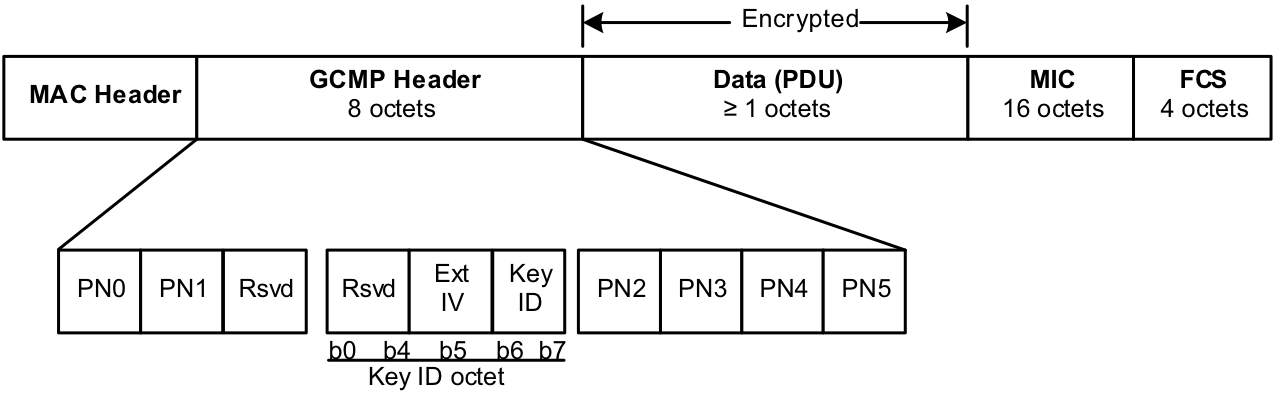
\includegraphics[width=\linewidth]{contents/background-in-wireless-networks/protected-network-standards/wpa3/gcmp/expanded-gcmp-mpdu.png}
    \caption{Expanded \gls{gcmp} \gls{mpdu}}
    {Source: \cite{ieee_80211_2020}}
    \label{figure:ieee80211_figure1226}
\end{figure}

Represented by Figure \ref{figure:ieee80211_figure1226}, the \gls{mpdu} of \gls{gcmp} is very similar to the \gls{ccmp} one, the \gls{mic} size being the only difference between them. Instead of a variant \gls{mic} size for 128-bit and 256-bit keys, \gls{gcmp}’s \gls{mic} is always 16-octet long.

\begin{figure}[h]
    \centering
    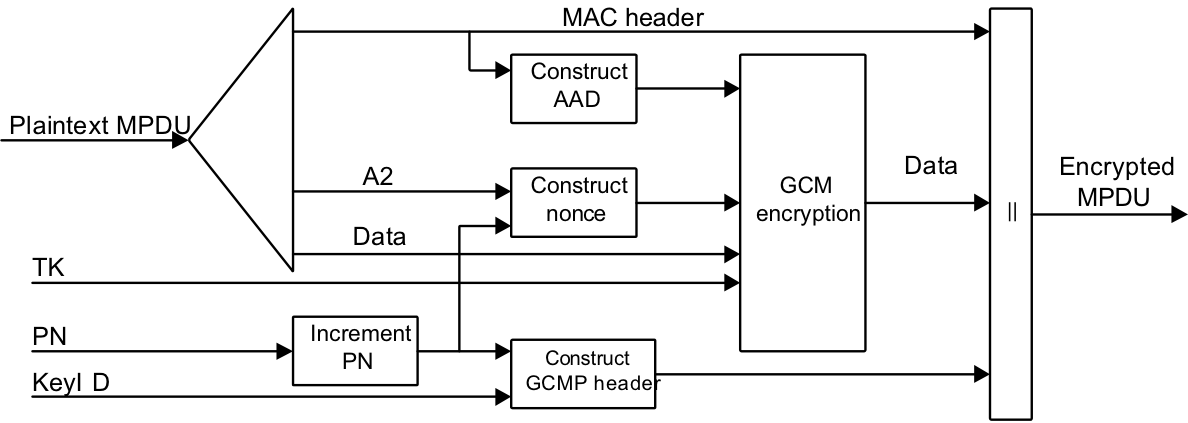
\includegraphics[width=\linewidth]{contents/background-in-wireless-networks/protected-network-standards/wpa3/gcmp/gcmp-encapsulation-block-diagram.png}
    \caption{\gls{gcmp} Encapsulation Block Diagram}
    {Source: \cite{ieee_80211_2020}}
    \label{figure:ieee80211_figure1227}
\end{figure}

The encapsulation process, shown on Figure \ref{figure:ieee80211_figure1227}, differs from \gls{ccmp} on the Nonce construction. The priority is no longer considered, only \gls{a2} and \gls{pn} still remain. As expected, the \gls{ccmp} Header construction is replaced with the \gls{gcmp} Header construction and the \gls{ccm} Originator Processing with the \gls{gcm} Originator Processing.

\begin{figure}[h]
    \centering
    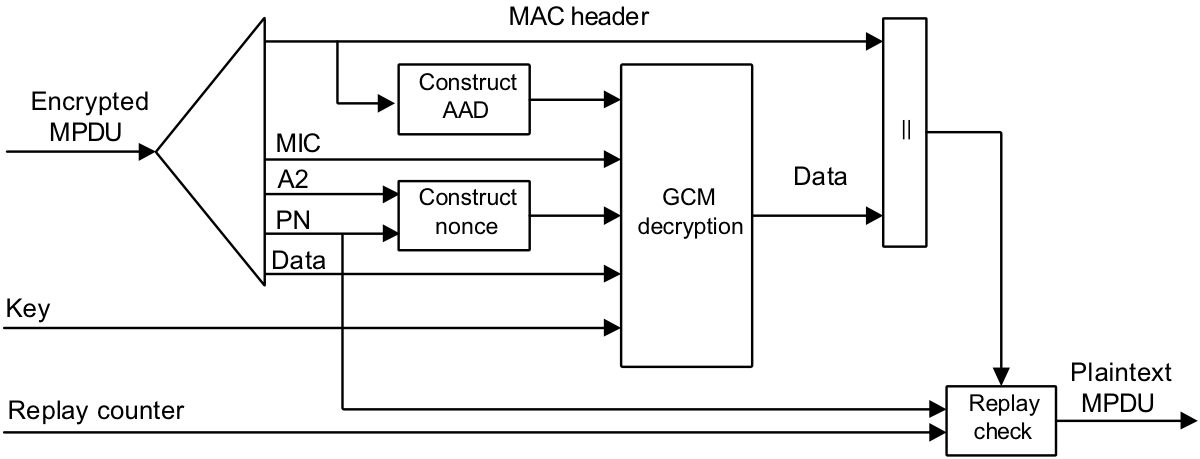
\includegraphics[width=\linewidth]{contents/background-in-wireless-networks/protected-network-standards/wpa3/gcmp/gcmp-decapsulation-block-diagram.png}
    \caption{\gls{gcmp} Decapsulation Block Diagram}
    {Source: \cite{ieee_80211_2020}}
    \label{figure:ieee80211_figure1229}
\end{figure}

On decapsulation, the \gls{ccm} Recipient Processing is substituted by the \gls{gcm} Recipient Processing. The Nonce construction is performed just like in the encapsulation process. The process is shown on Figure \ref{figure:ieee80211_figure1229}.

\FloatBarrier

\paragraph{Security}

A compromise was made on the \gls{tkip} design to make possible its use on legacy \gls{wep} hardware. The forgery attacks were mitigated with the introduction of the Michael algorithm, but, due to computing power constraints, while blocking the forged packets it would cause a denial of service on the network \cite{ieee_80211_2020}.

As \gls{tkip} just encapsulates the \gls{wep} algorithm, it still relies on the security of the \gls{rc4} \gls{prng}. It was found that the keystream generated by \gls{rc4} is biased towards certain sequences and it made practical attacks against \gls{wpa}-\gls{tkip} networks within an hour \cite{rc4nomore}. The attacker would establish a \gls{tcp} connection with some victim on the network and would repeatedly send identical packets particularly sized with a well-known content over the connection. Then the wireless traffic was captured and filtered to only what would likely be an attacker's packet. Ciphertext statistics were extracted and plaintext likelihoods calculated using a combination of the \gls{fm} and \gls{absab} biases. Finally, the \gls{mic} key is derived from one of the candidates with the correct \gls{icv}, allowing any other packet of the victim to be fully decrypted.

